\section{Stand der Technik}

\subsection{Grundlagen der Automatisierung in der Fertigung}
Die Automatisierung von Fertigungs- und Montageprozessen ist sehr wichtig für moderne Produktionssysteme. Ziel ist es, manuelle Tätigkeiten zu reduzieren, Prozessschritte zu standardisieren und eine gleichbleibende Produktqualität sicherzustellen sowie die Produktionskapazität zu erhöhen, indem mit derselben Personalstärke eine größere Anzahl von Einheiten hergestellt werden kann. Abhängig vom Automatisierungsgrad kommen dabei teilautomatisierte oder vollständig automatisierte Systeme zum Einsatz.

In der Montage werden automatisierte Systeme besonders dort eingesetzt, wo hohe Anforderungen an Wiederholgenauigkeit, Prozesssicherheit und Dokumentation bestehen. Automatisierung wird auch dort eingesetzt, wo der Mensch entlastet werden soll oder menschliche Arbeitskraft eingespart beziehungsweise gezielter für höherwertige, komplexe oder überwachende Tätigkeiten eingesetzt werden kann. Dies betrifft sowohl anspruchsvolle Montageaufgaben als auch stark repetitive und monotone Arbeitsprozesse.

Typische Anwendungsfelder sind das Positionieren von Bauteilen, das kontrollierte Einbringen von Kräften sowie das Verschrauben mit definierten Parametern. Neben der reinen Ausführung der Montageaufgaben spielt auch die Überwachung des Prozesses eine wichtige Rolle, um Abweichungen frühzeitig erkennen zu können.\cite{Groover_Automation,Lotter_Montage}

\subsection{Industrie 4.0 im Kontext der Montage}
Im Montageumfeld steht Industrie 4.0 vor allem für den Wandel von starren, fest definierten Abläufen hin zu flexiblen und vernetzten Montagesystemen. Maschinen, Werkzeuge und IT-Systeme sind miteinander verbunden und tauschen kontinuierlich Informationen aus. Dadurch lassen sich Montageschritte besser aufeinander abstimmen und Produktionsprozesse können schneller an neue Produkte, Varianten oder Stückzahlen angepasst werden. Diese Flexibilität gewinnt nicht nur bei kundenindividuellen Produkten, sondern auch bei hohen Stückzahlen zunehmend an Bedeutung.\cite{Kagermann_I40}

Ein weiterer zentraler Punkt ist der Umgang mit Daten. Während der Montage werden zahlreiche Prozessdaten erfasst, etwa zu Kräften, Zeiten oder Qualitätsmerkmalen. Diese Daten machen den Montageprozess transparenter und ermöglichen es, Schwachstellen zu erkennen und Abläufe schrittweise zu verbessern. Gleichzeitig verändert sich die Rolle des Menschen in der Montage: Digitale Assistenzsysteme können unterstützen, indem sie Informationen bereitstellen oder bei komplexen Arbeitsschritten helfen. Der Mensch bleibt dabei ein entscheidender Faktor, wird jedoch durch vernetzte und intelligente Systeme sinnvoll ergänzt.

Erste Elemente einer vernetzten Produktionsumgebung sind im Unternehmen bereits umgesetzt. Bei der SmarAct GmbH besteht eine Anbindung der Montage- und Prüfsysteme an das zentrale ERP-System. Die einzelnen Systeme greifen dabei auf im ERP hinterlegte Informationen zurück, beispielsweise auf Prüfparameter oder auftragsbezogene Vorgaben.

Durch diese Anbindung wird sichergestellt, dass die für einen Auftrag relevanten Parameter einheitlich und in aktueller Version an den jeweiligen System zur Verfügung stehen. Gleichzeitig entsteht eine durchgängige Verbindung zwischen Montage- und Prüfschritten, bei der Informationen systemseitig weitergegeben werden. Diese vorhandene Infrastruktur bildet eine sinnvolle Grundlage für eine weitergehende Automatisierung und Digitalisierung von Montageprozessen.

\subsection{Unternehmensprofil und Produktumfeld}
Die SmarAct GmbH entwickelt und fertigt hochpräzise Positioniersysteme mit Genauigkeiten im Nanometerbereich. Die Produkte kommen unter anderem in der Halbleitertechnik, Optik, Medizintechnik sowie in der Forschung zum Einsatz. Charakteristisch für diese Anwendungen sind hohe Anforderungen an Genauigkeit, Wiederholbarkeit und Langzeitstabilität.\cite{SmarAct_Company}

Ein wesentlicher Bestandteil des Produktportfolios sind die piezobasierten SMARSLIDE-Linearpionierer der Serie SLC, die auf dem Stick-Slip-Prinzip basieren. Diese Antriebstechnologie ermöglicht eine sehr hohe Positionierauflösung bei gleichzeitig kompakter Bauweise. Aufgrund der geringen Baugrößen und der engen Toleranzen stellen sowohl die Fertigung als auch die Montage dieser Systeme besondere Anforderungen an Präzision und Prozesssicherheit.

Die SLC-Serie ist in unterschiedlichen Bauformen erhältlich, die sich im Wesentlichen durch ihre Breite und Länge unterscheiden. Die SLC-17-Positionierer besitzen eine Breite von 17 mm und sind für Anwendungen mit besonders begrenztem Bauraum ausgelegt. Die SLC-24-Positionierer weisen eine Breite von 24 mm auf und bieten aufgrund ihrer größeren Bauform eine erhöhte mechanische Steifigkeit.

Zusätzlich unterscheiden sich die Positionierer hinsichtlich ihrer konstruktiven Ausführung. Die Standardausführung der SLC-Positionierer verfügt über eine sockel-förmige Bodenplatte. Ergänzend dazu wurden Varianten mit Wand entwickelt, um die mechanische Belastbarkeit zu erhöhen. Diese Ausführungen besitzen eine U-förmige Bodenplatte und wird als SLC-W bezeichnet.\cite{SmarAct_SLC}

Diese konstruktiven Unterschiede beeinflussen insbesondere den Aufbau der Linearführung sowie das erforderliche Vorspannkonzept. Darüber hinaus sind spezielle Ausführungen für den Einsatz im Hoch- und Ultrahochvakuum sowie unterschiedliche Materialkombinationen verfügbar.

\begin{figure}[htbp]
    \centering
    \begin{subfigure}[t]{0.48\linewidth}
        \centering
        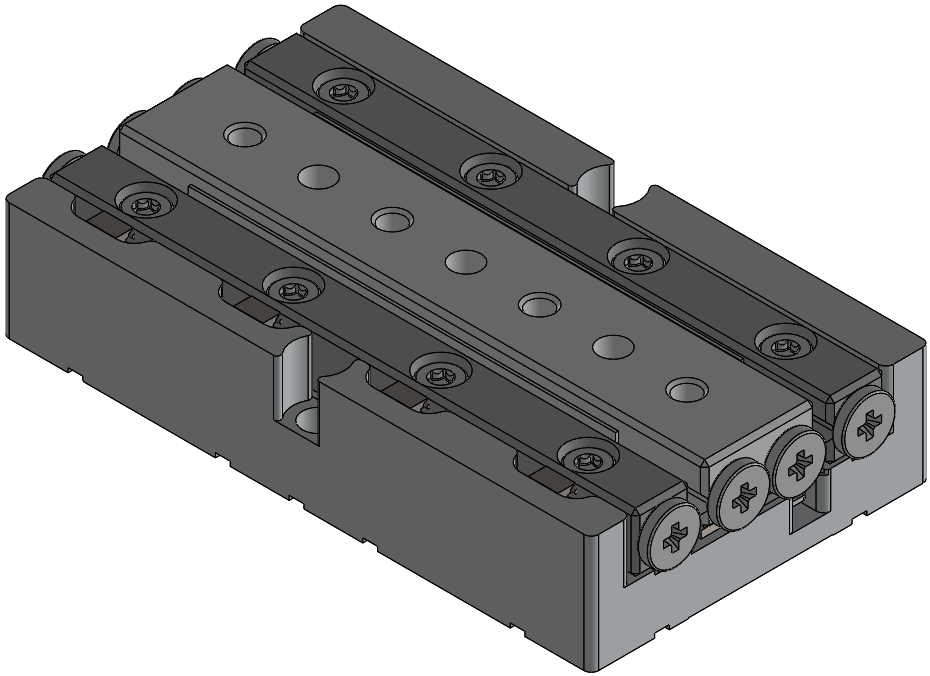
\includegraphics[width=\linewidth]{Bilder/02_Stand_der_Technik/SLC-1740-W.png}
        \caption{SLC-1740-W}
        \label{fig:slc1740_mit_wand}
    \end{subfigure}
    \hfill
    \begin{subfigure}[t]{0.48\linewidth}
        \centering
        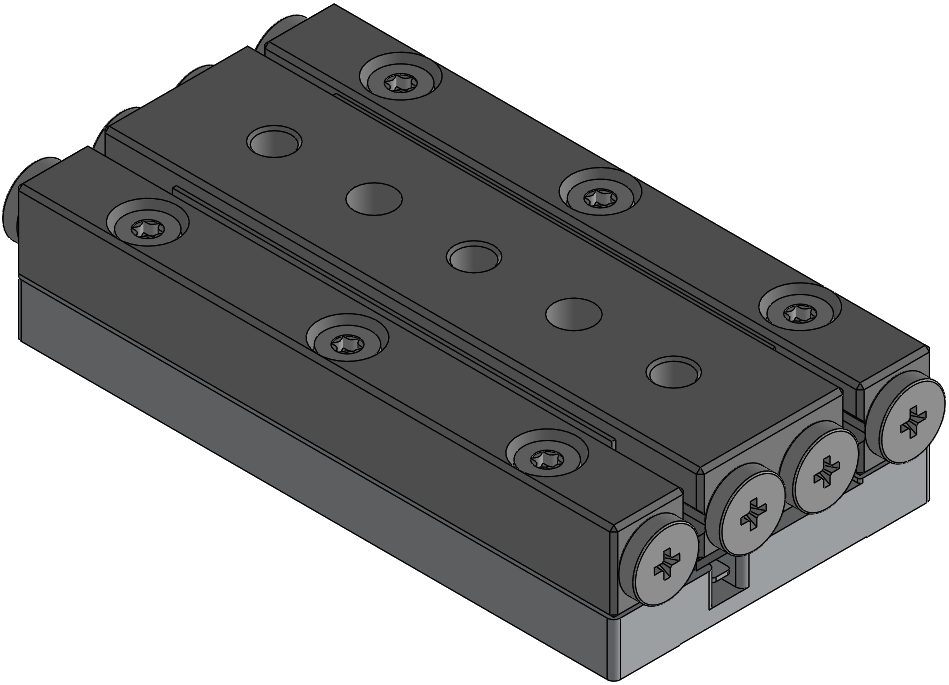
\includegraphics[width=\linewidth]{Bilder/02_Stand_der_Technik/SLC-2445.png}
        \caption{SLC-2445}
        \label{fig:slc2445}
    \end{subfigure}
    \caption{Bauformen der SLC-Positionierer mit unterschiedlichen Breiten und Bodenplattenausführungen (interne CAD-Daten)}
    \label{fig:slc_bauformen}
\end{figure}

\subsection{Aufbauprozess der SLC-Positionierer}
Der Aufbau der SLC-Positionierer erfolgt in mehreren aufeinander abgestimmten Montageschritten, bei denen insbesondere die Ausrichtung der Linearführung und die Einstellung der Vorspannung eine zentrale Rolle spielt.

Zu Beginn wird die Bodenplatte des Positionierers auf dem vorgesehenen Werkstückträger (auch Interface genannt) positioniert und fest verschraubt. Anschließend dient der Werkstückträger als Referenz- und Aufnahmeeinheit für die nachfolgenden Montageschritte, bei denen der vormontierte Piezoantrieb sowie die Positionssensorik (Encoder) mithilfe geeigneter Einbauhilfen in der Bodenplatte platziert und befestigt werden.

Diese Komponenten bilden die funktionale Basis des Positionierers und müssen bereits in dieser frühen Phase korrekt ausgerichtet sein, da spätere Korrekturen nur mit erheblichem Aufwand möglich sind.

Im nächsten Schritt wird der Schlitten gemeinsam mit den Kreuzrollen und dem Führungspaket auf die Bodenplatte aufgelegt. Eine Seite des Führungspakets wird dabei gezielt gegen eine vertikale, gerade Referenzfläche ausgerichtet. Dadurch wird sichergestellt, dass diese Seite des Führungspakets parallel zur Bodenplatte liegt. Anschließend wird die ausgerichtete Seite mit der Bodenplatte verschraubt.

\begin{figure}[htbp]
    \centering
    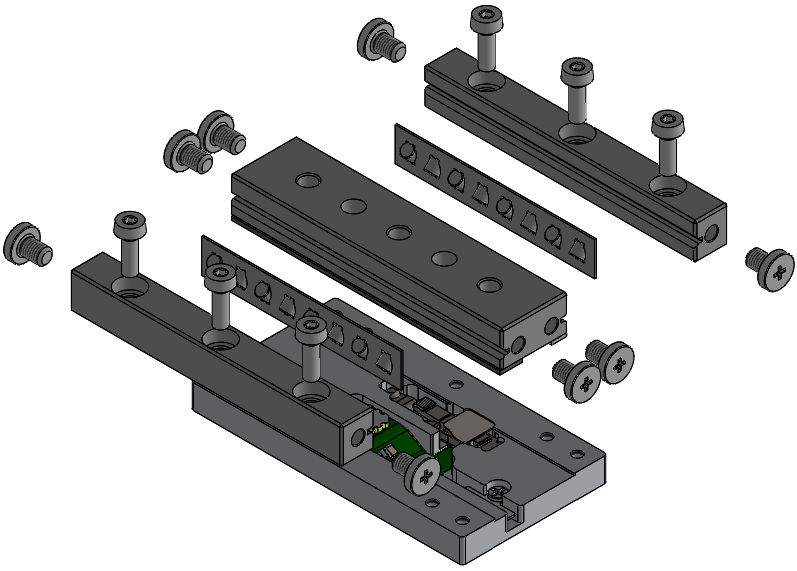
\includegraphics[width=0.5\linewidth]{Bilder/02_Stand_der_Technik/slc-explosion.png}
    \caption{Explosionsansicht der SLC-2445 Positionierer (basierend auf interne CAD-Daten)}
    \label{fig:slc2445_explosion}
\end{figure}

Nach diesem Montageschritt wird das Führungspaket vorgespannt, sodass das vorhandene Spiel zwischen Schlitten, Kreuzrollen und Führungselementen reduziert beziehungsweise vollständig eliminiert wird. Nach dem Einbringen der Vorspannung wird die gegenüberliegende Seite des Führungspakets verschraubt, wodurch die Position der Linearführung fixiert wird.

\subsection{Besonderheiten beim Aufbau von SLC-W-Positionierern}
Der grundlegende Aufbauprozess der SLC-W-Positionierer entspricht dem der Standard-SLC-Varianten. Der wesentliche Unterschied liegt in der Art und Weise, wie die Vorspannung eingebracht wird. Bei den Positionierern mit Wand erfolgt die Vorspannung nicht direkt über die Bodenplatte, sondern mithilfe von Keilen, die zwischen der Wand und einer Seite des Führungspakets positioniert werden.

Durch das gezielte Eindrücken dieser Keile wird eine definierte Vorspannkraft auf das Führungspaket aufgebracht. Die dabei von oben eingeleitete Kraft wird durch die Keilgeometrie in eine laterale Kraft auf das Führungspaket umgesetzt.

Beim anschließenden Verschrauben der gegenüberliegenden Seite ist es erforderlich, den Schlitten kontrolliert mitzubewegen. Dies ist erforderlich, da die angeordneten Rollenkäfige kürzer sind als die Gesamtlänge der Führung. Ohne ein Mitführen des Schlittens würde sich der wirksame Abstand zwischen den beiden Seiten des Führungspakets entlang der Führungsachse verändern.

Durch das gezielte Mitbewegen des Schlittens wird sichergestellt, dass der Abstand zwischen den beiden Seiten des Führungspakets über die gesamte Länge konstant bleibt und die Linearführung parallel ausgerichtet ist. Dadurch werden Verspannungen sowie geometrische Abweichungen innerhalb der Führung vermieden.

\begin{figure}[htbp]
    \centering
    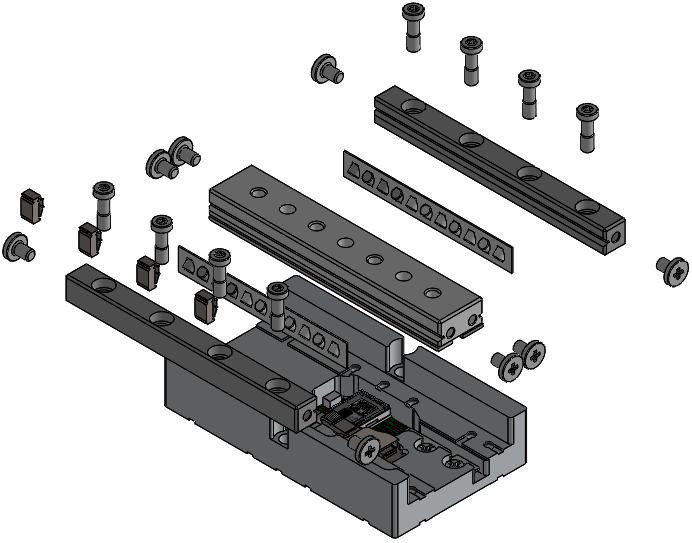
\includegraphics[width=0.5\linewidth]{Bilder/02_Stand_der_Technik/slc-w-explosion.png}
    \caption{Explosionsansicht der SLC-1740-W Positionierer (basierend auf interne CAD-Daten)}
    \label{fig:slc1740w_explosion}
\end{figure}

\subsection{Bedeutung der Vorspannung für die Funktion des Positionierers}
Die Vorspannung der Linearführung ist von entscheidender Bedeutung für die Funktion und Leistungsfähigkeit der SLC-Positionierer. Sie dient dazu, Roll-, Nick- und Gierbewegungen des Schlittens während der Bewegung durch den Piezoantrieb zu minimieren. Ohne eine korrekt eingestellte Vorspannung kann es zu Spiel innerhalb der Führung kommen, was sich unmittelbar negativ auf das Bewegungsverhalten auswirkt.\cite{Roloff_Matek}

Eine unzureichende Vorspannung kann zu verminderter Positioniergenauigkeit sowie reduzierter Steifigkeit führen. Darüber hinaus verschlechtert sich die Winkelgenauigkeit, insbesondere in Bezug auf Nick- und Gierbewegungen des Schlittens. Dies ist insbesondere bei Mikro- und Nanopositionieranwendungen kritisch, da selbst kleinste Abweichungen zu messbaren Positionsfehlern führen können.\cite{VDI2230}

Eine definierte und reproduzierbare Vorspannung ist daher eine grundlegende Voraussetzung für eine hohe Genauigkeit, stabile Bewegungsabläufe und eine zuverlässige Funktion der Positionierer. Aus diesem Grund stellt die Einstellung der Vorspannung einen besonders qualitätskritischen Montageschritt dar und ist von zentraler Bedeutung für eine mögliche Automatisierung des Aufbauprozesses.

Die Auswirkungen der Führungsgeometrie und der eingestellten Vorspannung lassen sich unter anderem anhand der Winkelabweichungen des Schlittens beschreiben.

\begin{figure}[htbp]
    \centering
    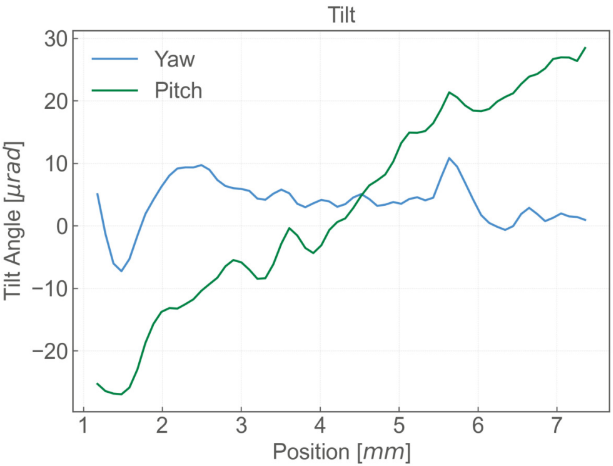
\includegraphics[width=0.5\linewidth]{Bilder/02_Stand_der_Technik/Vorspannung_Pitch_Yaw.png}
    \caption{Pitch- und Yaw-Abweichungen des Schlittens in Abhängigkeit vom Verfahrweg (basierend auf internen Produktdaten)}
    \label{fig:pitch_yaw_graph}
\end{figure}

Die in Abbildung~\ref{fig:pitch_yaw_graph} dargestellten Verläufe von Nicken (Pitch) und Gieren (Yaw) über den Verfahrweg zeigen, dass selbst geringe geometrische Abweichungen innerhalb der Linearführung messbare Winkeländerungen verursachen. Eine ungleichmäßige oder unzureichende Vorspannung kann diese Effekte verstärken und sich negativ auf die Positioniergenauigkeit auswirken.

\subsubsection{Ermittlung und Variation der Vorspannkräfte}
Zur Ermittlung der Vorspannkräfte wurden als Ausgangspunkt die vom Hersteller empfohlenen Einstellungen zur Vorspannung verwendet, die im Rahmen der Produktdokumentation intern zur Verfügung gestellt wurden. Diese basieren auf den angegebenen Einstellmomenten der Justierschrauben bzw. den dazugehörigen empfohlenen Vorspann-Einstellungen. Daraus wurde eine Referenz-Vorspannkraft $F_A$ (Herstellerwert) abgeleitet und als Vergleichsbasis festgelegt. Für die Versuche wurden die Kräfte anschließend gezielt variiert, um den Einfluss einer zu niedrigen bzw. zu hohen Vorspannung systematisch bewerten zu können.

Es wurde jeweils eine manuelle Vorspannung nach Arbeitsanweisung eingestellt, um eine praxisnahe Referenz zu erhalten. Danach wurden definierte Kraftstufen auf Basis von $F_A$ eingestellt ($F_A$, $1{,}5\cdot F_A$, $2\cdot F_A$, $2{,}5\cdot F_A$).

Für jede Stufe wurde derselbe Messablauf durchgeführt:
\begin{enumerate}
    \item Vorspannen
    \item Rollwiederstandsmessung
    \item Krafteinstellung
    \item Aktorvermessung
\end{enumerate}

Als Qualitätskennwerte wurden unter anderem Rollreibung, Krümmung (vertikal/horizontal), Umkehrfehler sowie Wiederholgenauigkeiten ausgewertet.

Die Ergebnisse zeigen, dass eine Erhöhung der Vorspannung zunächst zu einer deutlichen Reduktion von Spiel- und Umkehreffekten führt und damit insbesondere Umkehrfehler sowie die Wiederholgenauigkeit verbessert. Bei zu hoher Vorspannung nehmen jedoch einzelne Kennwerte wieder zu (z.\,B. durch steigende Reibung bzw. zusätzliche elastische Verformungen). Über beide Baugrößen hinweg lieferte eine Vorspannung von ungefähr $2\cdot F_A$ den besten Kompromiss aus geringer Rollreibung, stabiler Führungsgeometrie und guter Wiederholgenauigkeit. Diese Kraftstufe wurde daher als bevorzugter Zielwert für die weitere Auslegung des (automatisierten) Vorspannprozesses abgeleitet.

\subsection{Bestehende Montageprozesse im Unternehmen}
Der Aufbau der Linearführungen innerhalb der Positioniersysteme erfolgt derzeit überwiegend manuell. Die Montage umfasst das Aufsetzen der Führungen, das Einbringen der Vorspannelemente sowie das anschließende Verschrauben der Komponenten. Diese Arbeitsschritte erfordern ein hohes Maß an Sorgfalt und Erfahrung, da sie direkten Einfluss auf die Funktionalität des Endprodukts haben.

Die Einstellung der Vorspannung wird abhängig von der jeweiligen Bauform unterschiedlich realisiert. Für die Standardausführungen der SLC-Positionierer existiert bereits eine separate Vorspannvorrichtung, an der das Führungspaket manuell positioniert und vorgespannt wird. Die Vorrichtung besteht im Wesentlichen aus einem seitlich wirkenden Schieber, der das Führungspaket mit einer definierten Kraft zusammendrückt. Bei Positionierern mit Wand (SLC-W) wird die Vorspannung zusätzlich durch das Einbringen von Keilen erzeugt. Hierzu kommt ein Stößel zum Einsatz, der den jeweiligen Keil vertikal bis zu einer definierten Distanz in das System einpresst.

Abgesehen von diesen beiden Systemen erfolgt der überwiegende Teil des Montageprozesses händisch. Insbesondere das Ausrichten der Bauteile, das kontrollierte Verschrauben sowie die Überprüfung der Parallelität und Beweglichkeit des Schlittens liegen vollständig in der Verantwortung der ausführenden Person. Eine durchgängige Automatisierung oder Integration der einzelnen Montageschritte ist derzeit nicht gegeben.

\subsubsection{SLC-Vorspannsystem}
Das SLC-Vorspannsystem dient der gezielten Einstellung der seitlichen Vorspannung zwischen Führungspaket und Schlitten während des Montageprozesses. Es kommt als eigenständiges Vorspannsystem zum Einsatz und wird vor dem eigentlichen Schraubprozess verwendet.

Die Vorspannung wird über einen linear geführten Schieber realisiert, der das Führungspaket kontrolliert in Richtung des Schlittens verschiebt. Der Schieber ist mechanisch geführt und wird über eine Spindel mit Nut angetrieben, wodurch eine rein translatorische Bewegung mit definiertem Kraftangriff ermöglicht wird. Der maximale Verfahrweg des Vorspannsystems beträgt 49,5 mm und deckt damit alle erforderlichen Baugrößen innerhalb der SLC-Produktfamilie ab.

Während des Vorspannvorgangs wird das Führungspaket gegen den Schlitten gedrückt und in dieser Position gehalten. In diesem Zustand erfolgt der nachfolgende Schraubprozess, sodass die eingestellte Vorspannung während der Verschraubung konstant erhalten bleibt. Auf diese Weise wird sichergestellt, dass sich die Kontaktverhältnisse innerhalb der Linearführung nicht unkontrolliert verändern.

Der Kraftfluss innerhalb des Vorspannsystems erfolgt ausschließlich über starre mechanische Bauteile. Der Einsatz elastischer Elemente wird bewusst vermieden, um eine hohe Reproduzierbarkeit der eingestellten Vorspannung zu gewährleisten. Zur Erfassung und Überwachung der aufgebrachten Vorspannkraft ist eine Kraftmessdose direkt in den Kraftfluss integriert. Dadurch kann die eingeleitete Kraft messtechnisch erfasst und überprüft werden.

Zur Absicherung des Bewegungsbereichs sind zwei Gabellichtschranken als Endlagensensoren vorgesehen. Diese begrenzen den maximal zulässigen Verfahrweg des Schiebers und schützen das System vor mechanischer Überlastung.

Abbildung~\ref{fig:SLC_Vorspannsystem} zeigt das Vorspannsystem als eigenständige mechanische Baugruppe.

\begin{figure}[htbp]
    \centering
    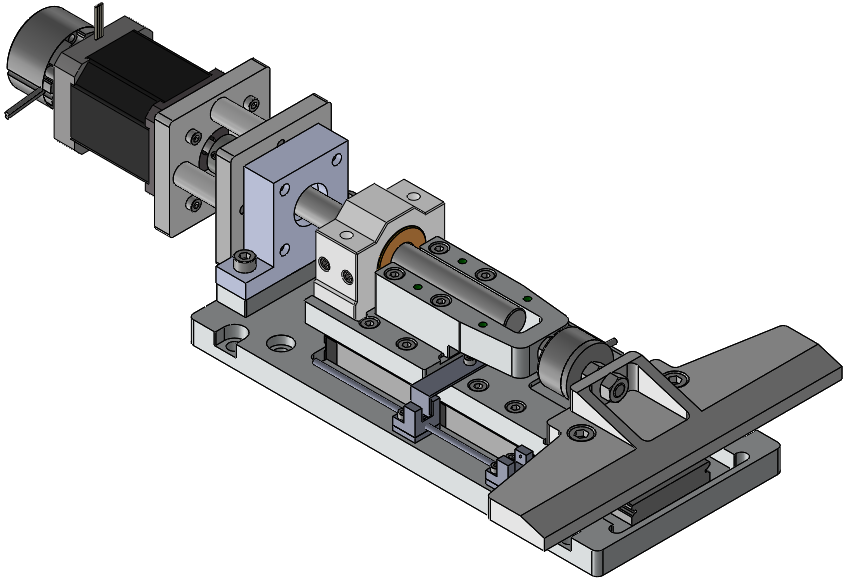
\includegraphics[width=0.5\linewidth]{Bilder/02_Stand_der_Technik/SLC_Vorspannen.png}
    \caption{Darstellung des SLC-Vorspannsystems}
    \label{fig:SLC_Vorspannsystem}
\end{figure}

\subsubsection{Keile-Einpresssystem}
Für Positionierer der Bauform SLC-W wird die Vorspannung zusätzlich über Keile eingestellt. Hierfür kommt ein separates Keileinpresssystem zum Einsatz, das den seitlichen Vorspannprozess ergänzt. Ziel dieses Systems ist es, die Keile kontrolliert und reproduzierbar in das Führungssystem einzubringen.

Der grundsätzliche Aufbau des Keileinpresssystems ist dem zuvor beschriebenen Vorspannsystem ähnlich, unterscheidet sich jedoch in der Bewegungsrichtung und der Art der Krafteinleitung. Während das Vorspannsystem eine seitlich wirkende Kraft auf das Führungspaket ausübt, erfolgt der Einpressvorgang beim Keilsystem vertikal. Der Keil wird dabei von oben in die vorgesehene Aufnahme eingepresst.

Die Bewegung des Einpressstempels erfolgt über einen linearen Aktor, der eine präzise Zustellung in Z-Richtung ermöglicht. Durch die lineare Führung wird sichergestellt, dass der Keil ohne Verkanten eingebracht wird und die Kraft senkrecht zur Führungsgeometrie wirkt. Der Einpressvorgang erfolgt ausschließlich translatorisch.

Zur Überwachung der aufgebrachten Einpresskraft ist eine Kraftmessdose direkt in den Kraftfluss integriert. Dadurch kann der Einpressvorgang kontrolliert überwacht und reproduzierbar durchgeführt werden.

Zur Absicherung des Bewegungsbereichs sind zwei Gabellichtschranken als Endlagensensoren vorgesehen. Diese erfassen die obere und untere Endlage des Einpressstempels und begrenzen den zulässigen Verfahrweg des Aktors. Dadurch wird ein sicherer Betrieb gewährleistet und gleichzeitig eine reproduzierbare Referenzierung des Systems ermöglicht.

\begin{figure}[H]
    \centering
    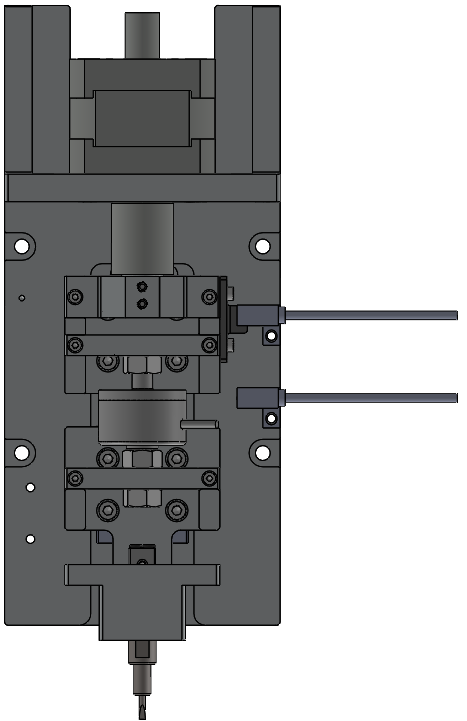
\includegraphics[width=0.5\linewidth]{Bilder/02_Stand_der_Technik/Keile_Einpress.png}
    \caption{Keile-Einpress System}
    \label{fig:keile_einpress}
\end{figure}

\subsection{Stand der Automatisierung im Unternehmen}
Der Automatisierungsgrad im Unternehmen unterscheidet sich deutlich zwischen Montage- und Testprozessen. Während der Aufbau der Positioniersysteme derzeit überwiegend manuell erfolgt, sind die nachgelagerten Prüfprozesse bereits in hohem Maße automatisiert.

Im Bereich der Montage existieren bislang lediglich einzelne, teilautomatisierte Hilfsmittel. Dazu zählen eine Vorspannvorrichtung für die Standardausführungen der SLC-Position\-ierer sowie eine separate Keileinpresssystem für Positionierer mit integrierter Wand (SLC-W). Diese Vorrichtungen unterstützen jeweils einzelne Prozessschritte, sind jedoch nicht miteinander verknüpft und nicht in einen durchgängigen Montageablauf integriert. Der Großteil der qualitätskritischen Tätigkeiten, wie das Ausrichten der Linearführung, das kontrollierte Einbringen der Vorspannung sowie das Verschrauben der Komponenten, wird weiterhin manuell durchgeführt. Die Qualität des Montageergebnisses hängt dabei in hohem Maße von der Erfahrung und Sorgfalt der ausführenden Person ab.

Demgegenüber ist der nachgelagerte Testprozess bereits weitgehend automatisiert und erlaubt eine reproduzierbare sowie strukturierte Erfassung der Funktions- und Qualitätsmerkmale der Positionierer. Der hohe Automatisierungsgrad im Testbereich verdeutlicht, dass insbesondere der Montageprozess aktuell den verbleibenden manuellen und qualitätskritischen Abschnitt innerhalb der Prozesskette darstellt und damit ein zentrales Potenzial für eine weitere Automatisierung bietet.

\subsection{Einordnung der Arbeit in den Stand der Technik}
Die vorliegende Arbeit ist im Spannungsfeld zwischen hochautomatisierten Testprozessen und weitgehend manuellen Montageabläufen einzuordnen. Während im Unternehmen bereits umfangreiche Erfahrungen mit der Automatisierung komplexer Prüfprozesse bestehen, sind qualitätskritische Montageschritte bislang nur begrenzt standardisiert und reproduzierbar.

Ziel dieser Arbeit ist es, den Montageprozess der Linearführungen von SLC-Positionierern in seinen qualitätskritischen Teilschritten zu verstehen und daraus ein automatisierbares Montagekonzept abzuleiten. Im Vordergrund stehen dabei die reproduzierbare Einstellung der seitlichen Vorspannung sowie das nachfolgende Fixieren der seitlichen Führungselemente. Ergänzend werden die notwendigen Prozessschnittstellen beschrieben, die eine strukturierte Bauteilführung, ein definiertes Referenzieren und eine sichere Handhabung während der Montage ermöglichen.

Durch die Entwicklung eines modularen und erweiterbaren Montagekonzepts soll ein Beitrag zur schrittweisen Erhöhung des Automatisierungsgrads geleistet werden. Gleichzeitig ermöglicht das Konzept eine verbesserte Prozesskontrolle und Dokumentation qualitätsrelevanter Parameter (z. B. Vorspannkraft und Schraubparameter). Die Arbeit überträgt damit etablierte Prinzipien der Automatisierung der Fertigung gezielt auf die spezifischen Anforderungen hochpräziser Positioniersysteme der SmarAct GmbH.